\documentclass[11pt,xcolor=dvipsnames,aspectratio=169]{beamer}

\mode<presentation>
{
  \useinnertheme{circles} 
  \usecolortheme[named=Black]{structure} 
  \setbeamertemplate{navigation symbols}{}
  \setbeamertemplate{footline}[page number]
  \setbeamercovered{transparent}
}

\usepackage{physcomm}

%\usepackage{adjustbox}
\usepackage[export]{adjustbox}
\usepackage{graphicx}
\usepackage{colortbl}
\usepackage{pifont}
\usepackage{amsmath}
\usepackage{scrdate,scrtime}
\usepackage{subfig}
\usepackage{verbatim}
\usepackage{booktabs}
\usepackage{rotating}
\usepackage{xspace}
\usepackage{xcolor}
\usepackage{bm}
\usepackage{pdfpages}
\usepackage{enumerate}
\usepackage{amsmath}
\usepackage{xspace}
\usepackage{ifthen}
 
%-----------------------------------------------------------------------
% custom colors 
\definecolor{EDBRed}{RGB}{220,20,60} 
\definecolor{EDBDarkBlue}{RGB}{0,0,160}
\definecolor{EDBBlue}{RGB}{0,135,189}
\definecolor{EDBGray}{RGB}{211,211,211}

%-----------------------------------------------------------------------
% text boxes 
\usepackage{tcolorbox}
%\usepackage{mdframed}

% 1- Block title (background and text)
\setbeamercolor{block title}{bg=EDBBlue!60, fg=black}
% 2- Block body (background)
\setbeamercolor{block body}{bg=EDBBlue!60}

\setbeamercolor{block title alerted}{fg=white, bg=orange}
% 2- Block body (background)
\setbeamercolor{block body alerted}{bg=orange!25}

% 1- Block title (background and text)
\setbeamercolor{block title example}{fg=white, bg=teal}
% 2- Block body (background and text)
\setbeamercolor{block body example}{bg=EDBBlue!60}

% arrows between color boxes
\usepackage{tikz}
\usetikzlibrary{arrows.meta, % for arrows style
                positioning  % for positioning of boxes
               }

%-----------------------------------------------------------------------
% backup 
\newcommand{\backupbegin}{
   \newcounter{framenumberappendix}
   \setcounter{framenumberappendix}{\value{framenumber}}
    \setbeamertemplate{footline}{
   \leavevmode%
   \hbox{%
   \begin{beamercolorbox}[wd=1.00\paperwidth,ht=0.01ex,dp=1ex,right]{} 
     {\normalsize \insertframenumber{}} \hspace{0.065\textwidth}
   \end{beamercolorbox}
   }%
   \vskip0pt%
 }
}

\newcommand{\backupend}{
   \addtocounter{framenumberappendix}{-\value{framenumber}}
   \addtocounter{framenumber}{\value{framenumberappendix}} 
}

% -----------------------------------------------------------------------
% slide layout & footnotes
\setbeamertemplate{frametitle}{ 
%\begin{centering} 
\vspace{0.03\paperheight}
{\huge \insertframetitle }
\vspace{0.01\paperheight}
\par 
%\end{centering} 
}


%\setbeamertemplate{footline}[text line]{%
%\parbox{\linewidth}{\small \vspace*{-10pt} \ \hfill \ \insertpagenumber / \inserttotalframenumber}}

\setbeamertemplate{footline}[text line]{%
\parbox{\linewidth}{\small \vspace*{-10pt} \ \hfill \ \insertframenumber / \inserttotalframenumber}}

\let\footnoterule\relax

\newcommand\blfootnote[1]{%
  \begingroup
  \renewcommand\thefootnote{}\footnote{\hspace{-30pt}\textcolor{Gray}{\tiny #1}}%
  \addtocounter{footnote}{-1}%
  \endgroup
}

% -----------------------------------------------------------------------
% itemize margins
\setlength{\leftmargini}{0.025\linewidth}
\setlength{\leftmarginii}{0.021\linewidth}

% sub-item size:
\setbeamerfont{itemize/enumerate subbody}{size=\normalsize} %to set the body size
%\setbeamertemplate{itemize subitem}{\normalsize\raise1.25pt\hbox{\donotcoloroutermaths$\blacktriangleright$}}  %to set the symbol size 
% -----------------------------------------------------------------------
\begin{document}

{
\usebackgroundtemplate{
\includegraphics[width=\paperwidth]{background/template_169_logos.pdf}}%
\begin{frame}[noframenumbering,plain]
  \begin{center}
    \setlength{\parskip}{0pt}
    \vspace{10pt}
    {\Huge\bf Deep Learning \& the Higgs Boson}\\[0.1\textheight]
    {\huge \bf Dr. Liza Mijovi\'c}
  \end{center}
\end{frame}
}

{
\usebackgroundtemplate{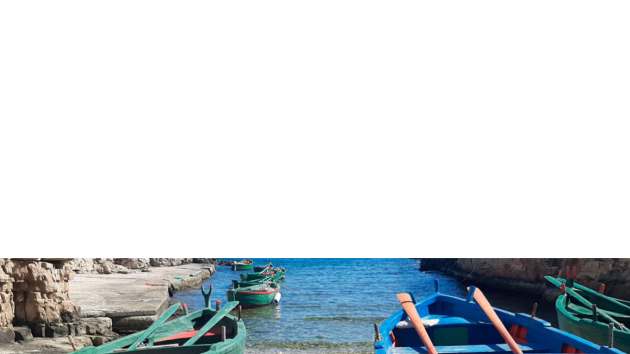
\includegraphics[width=\paperwidth]{background/template_169.pdf}}%
\begin{frame}[plain]
  \frametitle{\bf Deep Learning \& the Higgs Boson}
  \adjustbox{valign=t}{\begin{minipage}[t][0.55\textheight]{\linewidth}
      Classification with Fully Connected and Adversarial Networks.
      \vfill
      \begin{itemize}
      \item {\bf Lecture1: The Higgs boson and event classification:}\\
        - Event classification with a fully connected neural network (NN) with Keras API.\\
      \end{itemize}
      \vfill
      \begin{itemize}      
      \item {\bf Lecture2: Solving the background sculpting challenge:}\\
        - Event classification with adversarial neural network (ANN).\\
        - Hands-on knowledge of manipulating neural networks in Tensorflow.
      \end{itemize}
      \vfill
      \begin{itemize}          
      \item {\bf Lecture3: Putting it all together:}\\
        - Compare ANN classification performance to the fully connected network.
      \end{itemize}
      \vfill
\end{minipage}}
% vertical place-holder
\adjustbox{valign=t}{\begin{minipage}[t][0.35\textheight]{\linewidth} 
  \end{minipage}}
\end{frame}
}


{
\usebackgroundtemplate{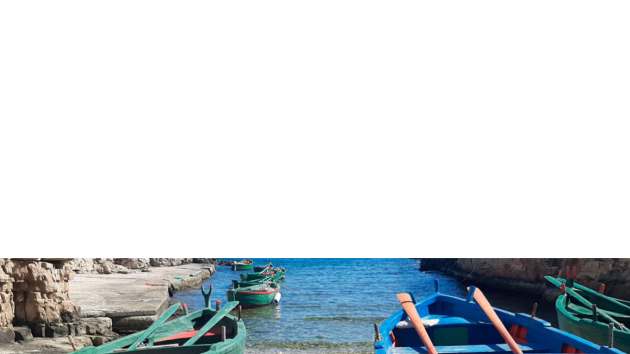
\includegraphics[width=\paperwidth]{background/template_169.pdf}}%
\begin{frame}[plain]
  \frametitle{\bf Lecture2:  classification with adversarial neural network}
  \adjustbox{valign=t}{\begin{minipage}[t][0.55\textheight]{\linewidth}
      \vfill
      \begin{itemize}
      \item {\bf What were we doing in Lecture1?}\\
        Classification with fully connected neural network.  
      \end{itemize}
      \begin{itemize}
      \item {\bf What is the issue with classification from Lecture1?}\\
        The discriminant has an undesired bias. 
      \end{itemize}
      \begin{itemize}
      \item {\bf How do we solve this issue?}\\
        Classification with adversarial neural network (ANN).
      \end{itemize}        
      \vfill
\end{minipage}}
% vertical place-holder
\adjustbox{valign=t}{\begin{minipage}[t][0.35\textheight]{\linewidth} 
  \end{minipage}}
\end{frame}
}

\begin{frame}
  \frametitle{\bf Any problems during lecture1?}
  When running:\\
  {\tt conda create --name DeepLearn23 --file requirements.txt}\\
  conda could not resolve the environment. 
  \begin{figure}
    \includegraphics[width=0.55\textwidth]{figures/l2/req.png}
  \end{figure}
  Solution: remove package versions. Ie {\tt jupyter=1.0.0=py39h06a4308\_7}
  becomes {\tt jupyter} etc.
\end{frame}


\begin{frame}
  \frametitle{\bf Reminder: Our Challenge}

  \adjustbox{valign=t}{\begin{minipage}[c]{0.5\linewidth}
      \vfill
        {\bf Classification: separate}
        \begin{itemize}
        \item \textcolor{EDBRed}{Signal} with Higgs boson.
        \item \textcolor{EDBBlue}{Background} with no Higgs boson.
        \end{itemize}
        \vfill
        {\bf Approach:} 
        \begin{itemize}
        \item use synthetic data.
        \item \textcolor{EDBBlue}{Introduce no bumps in the \myy{} distribution;
            these would hamper the background estimate.\\
            $\Rightarrow$ this lecture.}
        \end{itemize} 
      \end{minipage}}
    \adjustbox{valign=t}{\begin{minipage}[c]{0.49\linewidth}     
      \begin{figure}
        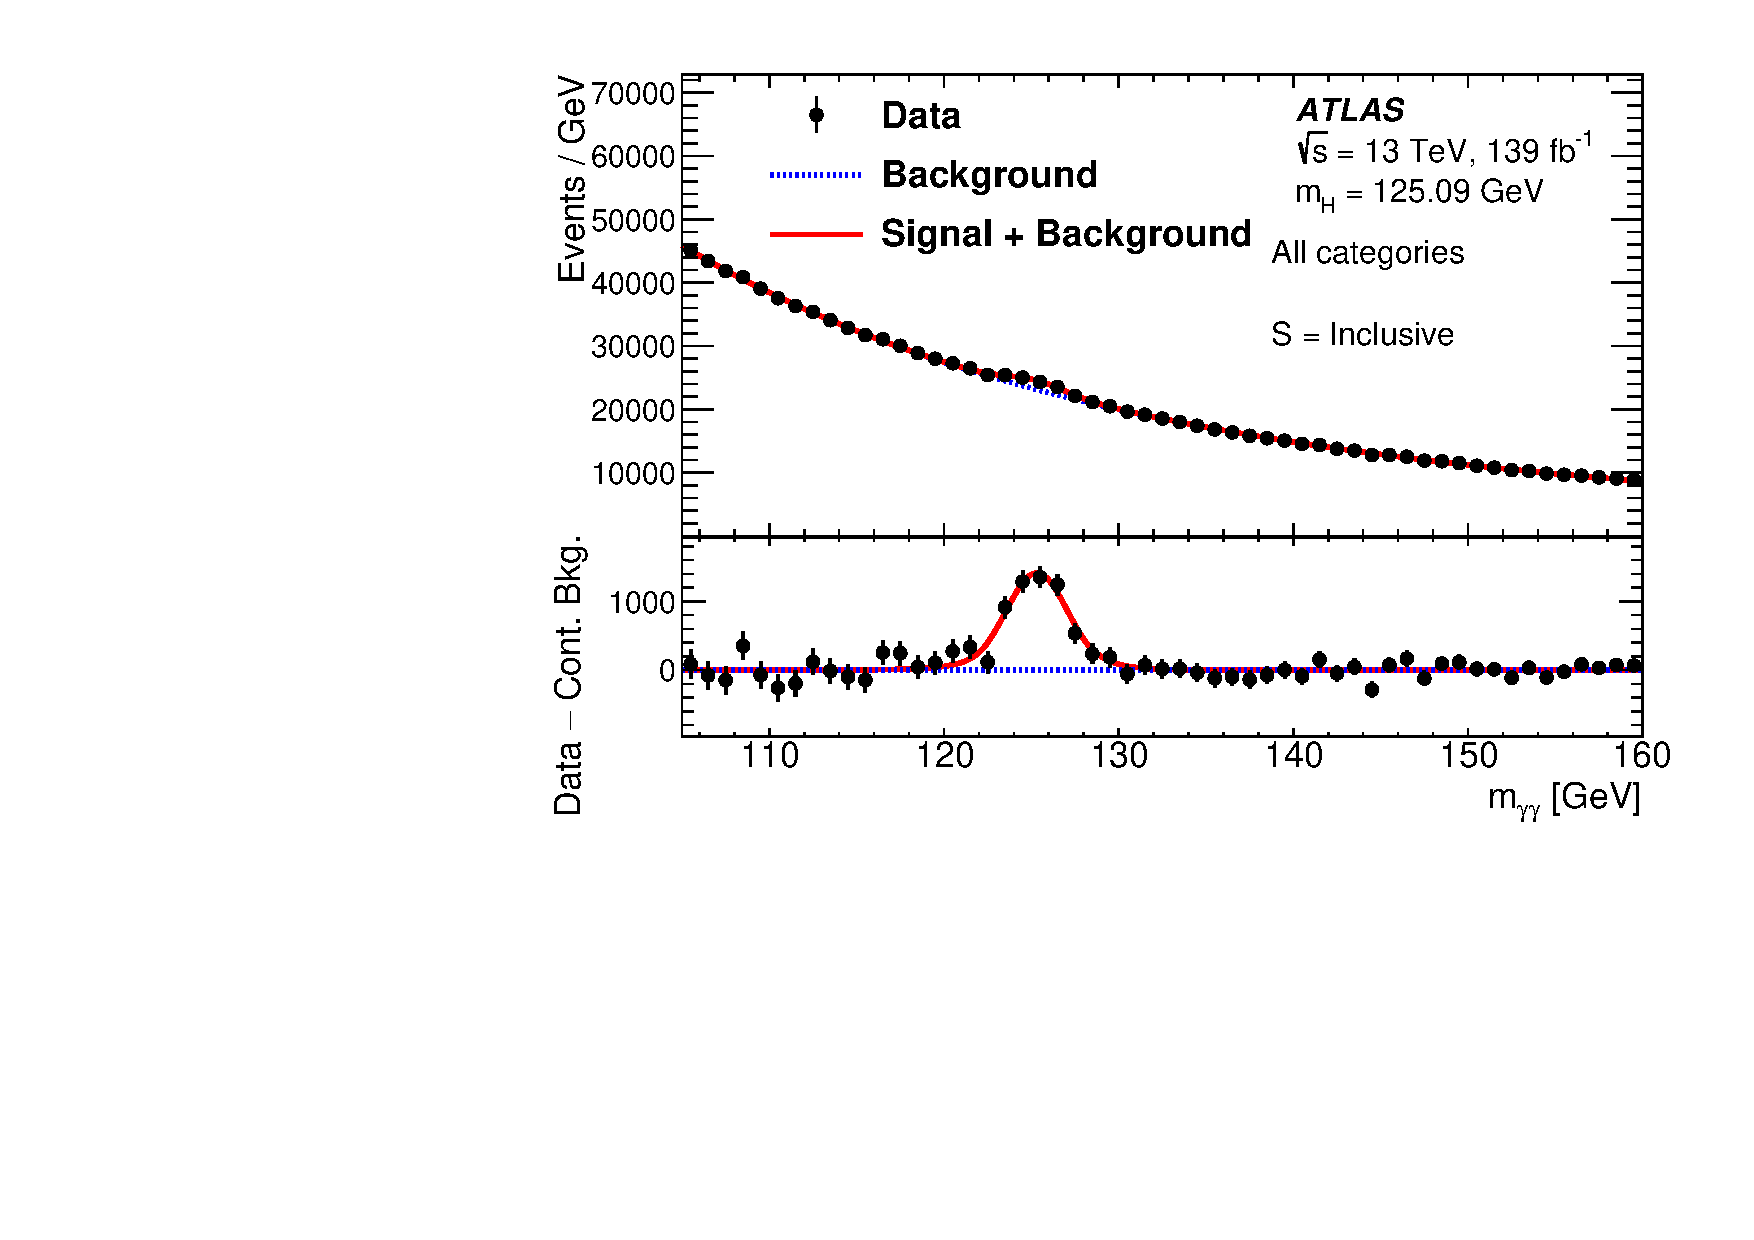
\includegraphics[width=1.00\textwidth]{figures/l1/challenge/figaux_01.pdf}
      \end{figure}
    \end{minipage}}
   \blfootnote{\scriptsize{L. Mijovi\'c, ATLAS, \href{https://arxiv.org/abs/2207.00348}{JHEP (2022)}.}}  
\end{frame}


\begin{frame}
  \frametitle{\bf Reminder: What is in the data?}
  \begin{center}
    Two photons ($\gamma$) per event, with momenta $p$.\\
    \vspace{20pt}
  \textcolor{EDBRed}{\Large Signal, label=1} \hspace{0.25\textwidth}
  \textcolor{Blue}{\Large Background, label=0}
  \end{center}
      \begin{figure}
        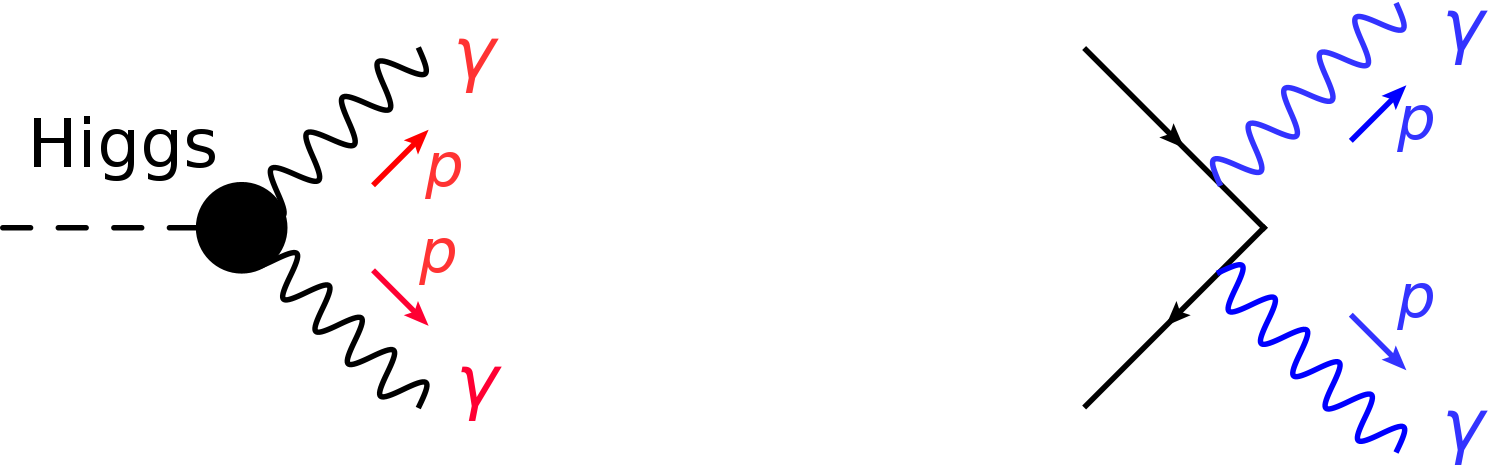
\includegraphics[width=0.80\textwidth]{figures/l1/challenge/SvsB.png}
      \end{figure}     
\end{frame}

\begin{frame}
  \frametitle{\bf Reminder: What is in the data?}
  \begin{itemize}
  \item Momenta $p$ are  4-dimensional (Lorentz) vectors.
  \item They are passed in cylindrical coordinates.
  \end{itemize}
  \begin{figure}
    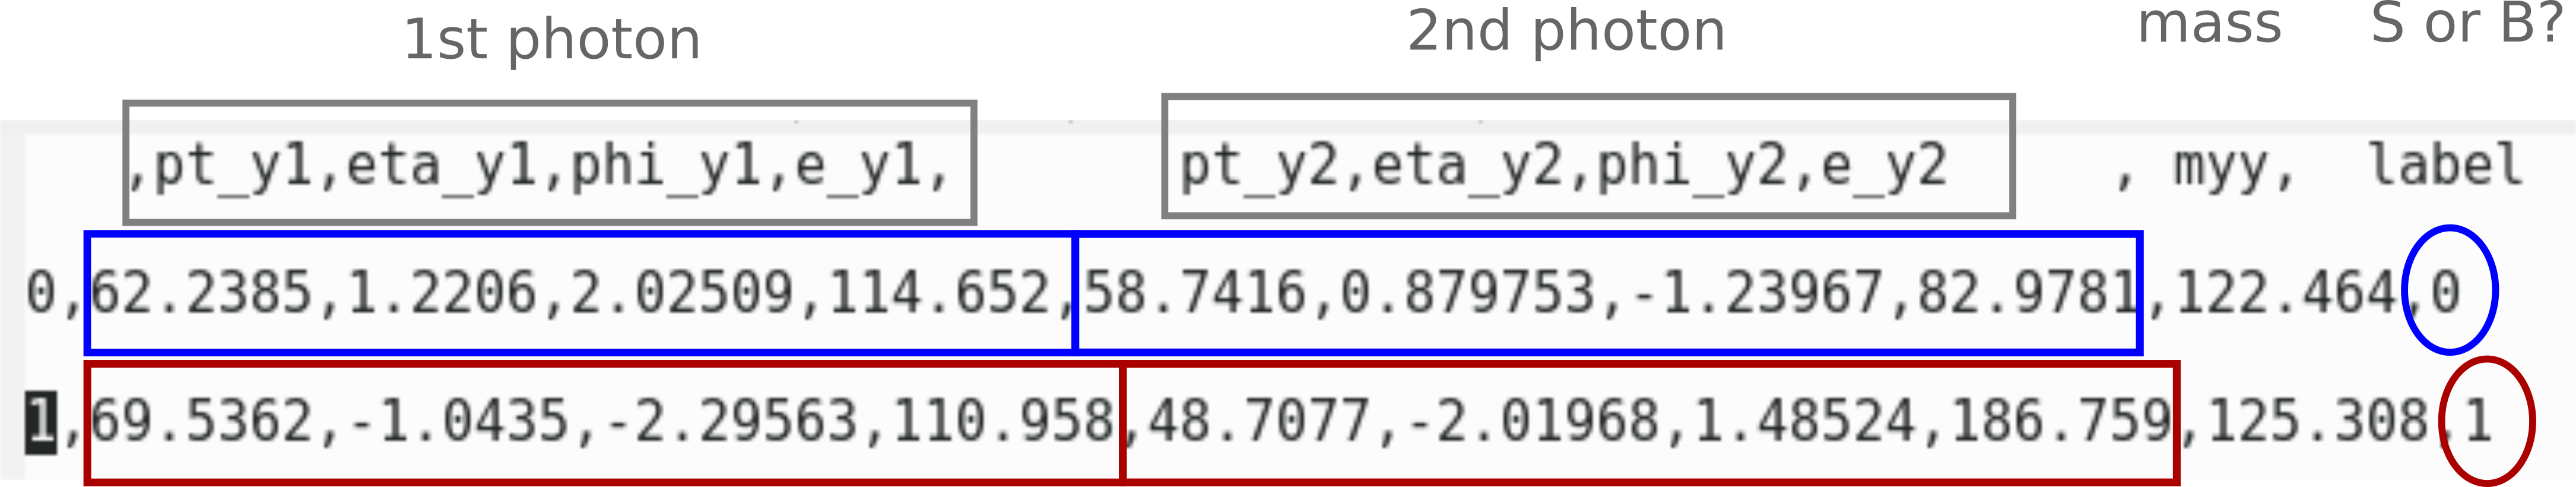
\includegraphics[width=1.00\textwidth]{figures/l1/challenge/data_annot.png}
  \end{figure}
\end{frame}

\begin{frame}
  \frametitle{\bf Lecture1: Classification}
  \adjustbox{valign=c}{\begin{minipage}[c]{0.49\linewidth}
      Fully connected deep neural network.\\
      {\bf Inputs:}
        \begin{itemize}
        \item Features $x$: photon 4-vectors.
        \item Labels $y$: signal (1) or background (0).
        \end{itemize}
        {\bf Training:}
        \begin{itemize}
        \item Combine 8 inputs into 1 classifier.
        \item Objective: minimise classifier loss $L_{clf}$.
        \item Training determines node weights $\theta_{clf}$.
        \end{itemize}
        {\bf Output:}
        \begin{itemize}
        \item discriminant: $z = p_{clf}(y|x,\theta_{clf})$.
        \end{itemize}
    \end{minipage}}
    \adjustbox{valign=c}{\begin{minipage}[c]{0.45\linewidth}     
      \begin{figure}
                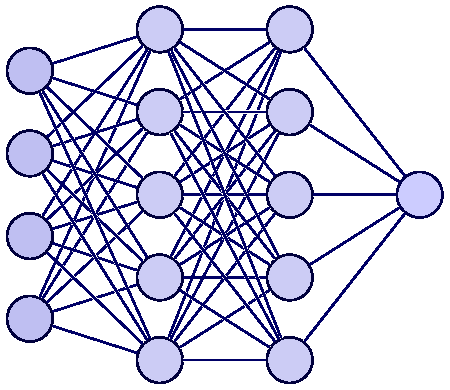
\includegraphics[width=1.00\textwidth]{figures/l2/class.pdf}
      \end{figure}
    \end{minipage}}
\end{frame}

\begin{frame}
  \frametitle{\bf Lecture1: Classification Results}
  We can separate \textcolor{EDBRed}{Signal} from \textcolor{Blue}{Background}.
  \begin{figure}
    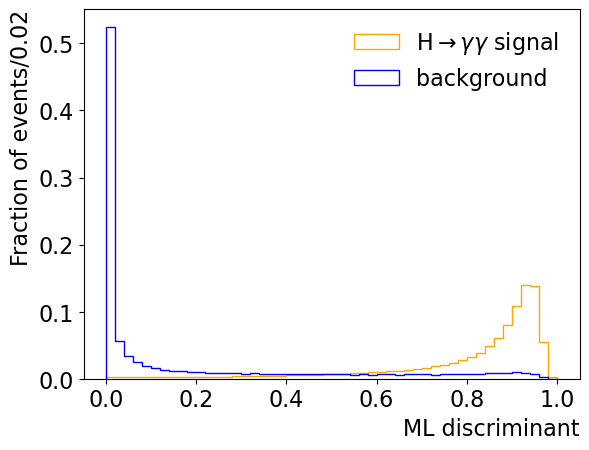
\includegraphics[width=0.49\textwidth]{figures/l2/discriminant.png}
    \includegraphics[width=0.49\textwidth]{figures/l2/myy_bonly.png}    
  \end{figure}
  However: \textcolor{Blue}{Background} grows a bump at \textcolor{Orange}{high discriminant values.}
\end{frame}


\begin{frame}
  \frametitle{\bf Lecture1: Classification Issue}
  We can separate \textcolor{EDBRed}{Signal} from \textcolor{Blue}{Background}.\\
  However: \textcolor{Blue}{Background} grows a bump at \textcolor{Orange}{high discriminant values.}
  \begin{figure}
    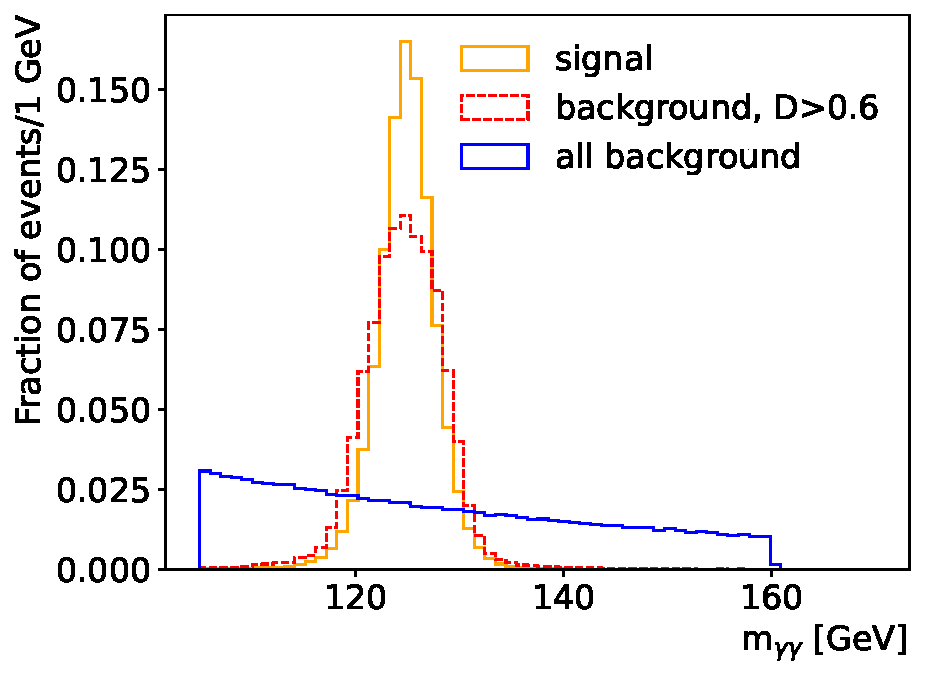
\includegraphics[width=0.45\textwidth]{figures/l2/lect_plots/myy_noscale.pdf}
    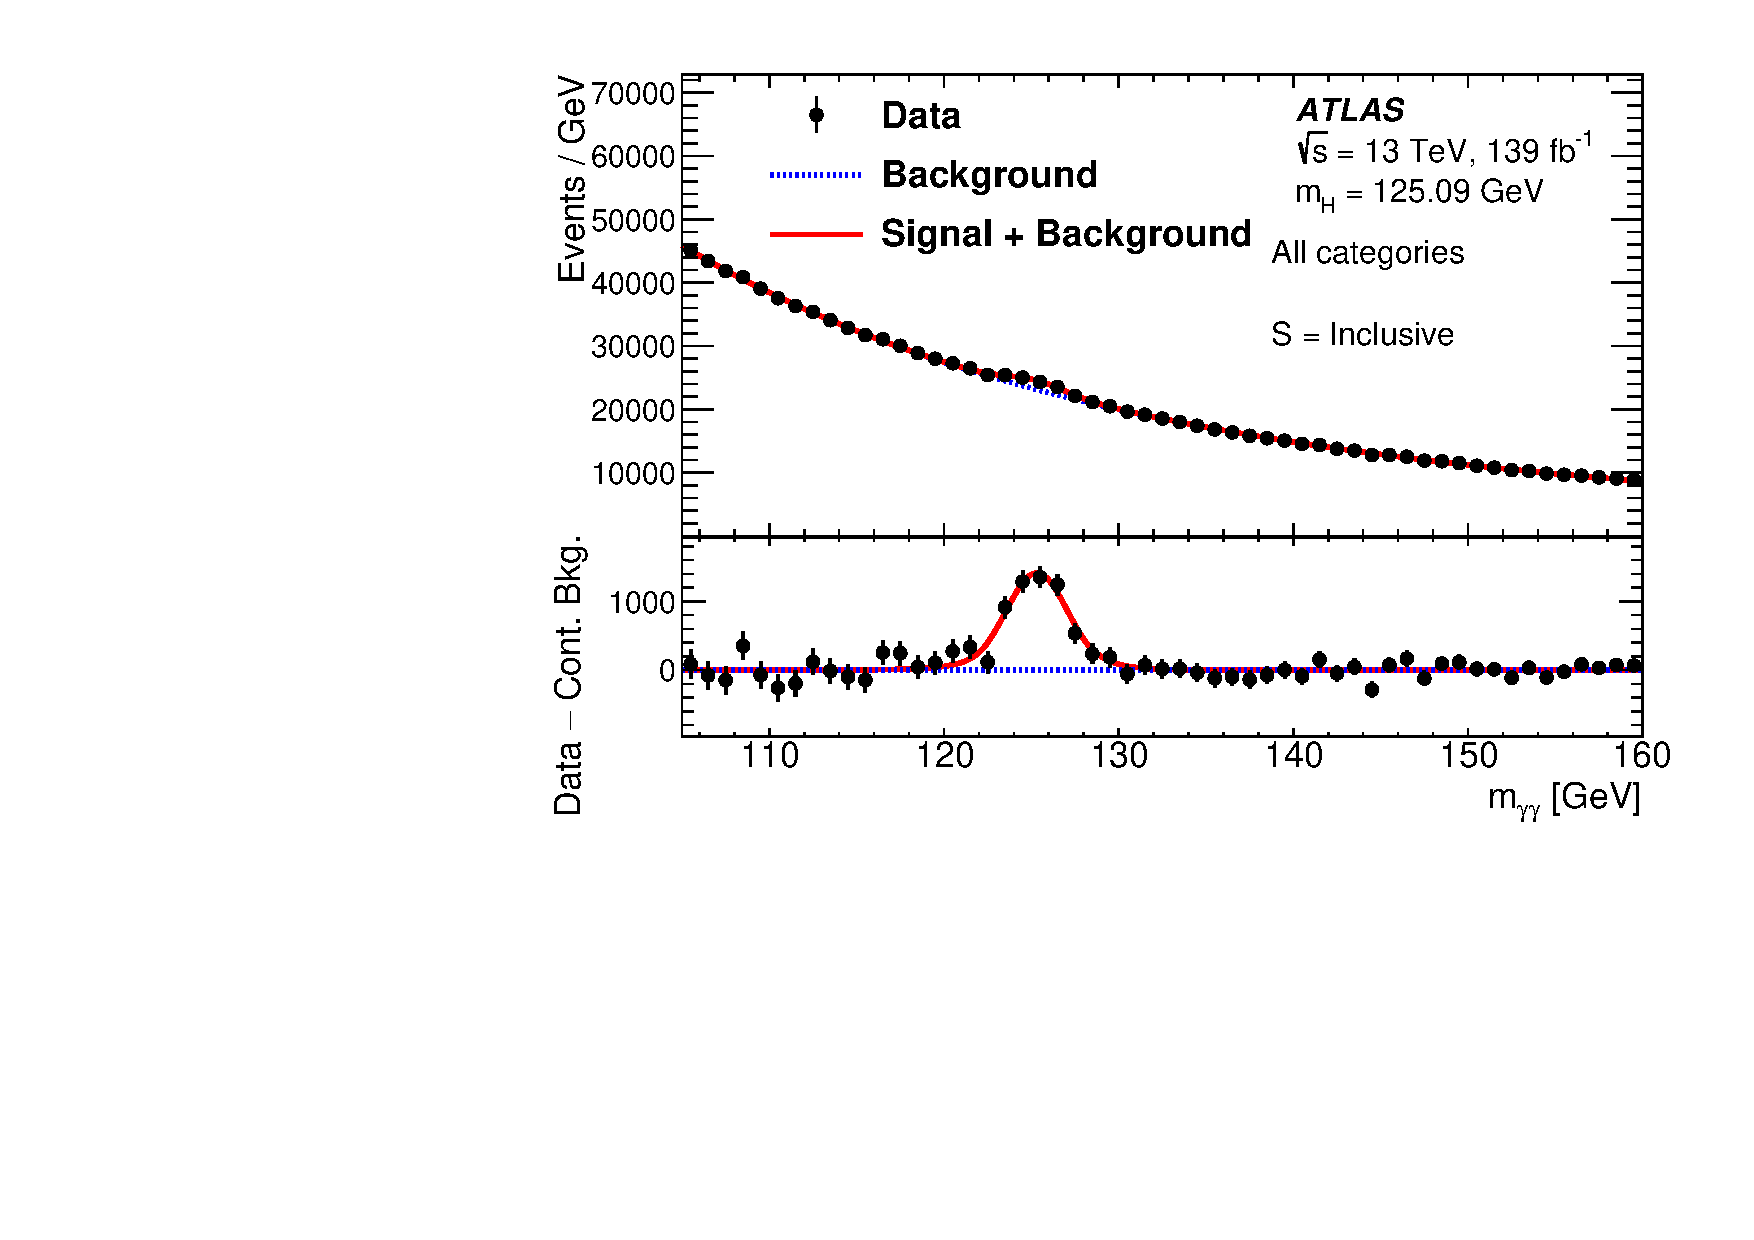
\includegraphics[width=0.49\textwidth]{figures/l1/challenge/figaux_01.pdf}
  \end{figure}
  This would prevent us from reliably estimating the background.\\
  Can we design classification which does not sculpt \myy{}? 
\end{frame}

\begin{frame}
  \frametitle{\bf Adversarial Neural Network}
  Can we design classification which does not sculpt \myy{}?
  \begin{itemize}
  \item Pit \textcolor{EDBBlue}{classifier} network against \textcolor{EDBRed}{adversary}.
  \item \textcolor{EDBBlue}{Classifier} tries to guess event label $y$ (0 or 1) from inputs $x$.
  \item \textcolor{EDBRed}{Adversary} tries to guess $\myy$ from classifier output.
  \item If possible, the \textcolor{EDBBlue}{classifier} is penalised.
  \end{itemize}
  \begin{figure}
    \includegraphics[width=1.0\textwidth]{figures/l2/and_ann.png}
  \end{figure}
  \blfootnote{Adapted from: A. Sogaard's,
    \href{https://github.com/asogaard/ep2mlf/blob/master/01-adversarial/2018-11-13_EP2MLF_AndreasSogaard.pdf}{lecture
    on adversarial NN.}}
\end{frame}

\begin{frame}
  \frametitle{\bf Gaussian Mixture Model}
  \begin{itemize}
  \item \textcolor{EDBRed}{Adversary} tries to guess $\myy$ from classifier output.
  \item If possible, the \textcolor{EDBBlue}{classifier} is penalised.
  \end{itemize}
  {\bf Q:} How do we know if the adversary is guessing the myy?\\
  {\bf A:} Gaussian Mixture Model (GMM).
  \begin{figure}
    \includegraphics[width=0.49\textwidth]{figures/l2/and_adv.png}
    \includegraphics[width=0.49\textwidth]{figures/l2/gmm.png}
  \end{figure}
  \blfootnote{Image credits: A. Sogaard, and
    \href{http://dx.doi.org/10.1016/j.ultrasmedbio.2019.01.018}{Ultrasound in
      Medicine \& Biology 45 (5) (2019).}}
\end{frame}

\begin{frame}
  \frametitle{\bf Mass decorrelation: gradient reversal}
  Can we design classification which does not sculpt \myy{}?
  \begin{itemize}
  \item \textcolor{EDBRed}{Adversary}: parametrises $d=\myy{}$ conditional on classifier output; $p_{adv}(\myy{}|z).$
  \item Trained with: \textcolor{EDBRed}{adversary loss $L_{adv}(\theta_{adv})$}.
  \item Gradient minimising \textcolor{EDBRed}{$L_{adv}$} is back-propagated to
    \textcolor{EDBBlue}{classifier}: gradient reversal layer.
  \end{itemize}
  \begin{figure}
    \includegraphics[width=1.0\textwidth]{figures/l2/and_ann.png}
  \end{figure}
  \blfootnote{Adapted from: A. Sogaard's,
    \href{https://github.com/asogaard/ep2mlf/blob/master/01-adversarial/2018-11-13_EP2MLF_AndreasSogaard.pdf}{lecture
    on adversarial NN.}}
\end{frame}


\begin{frame}
  \frametitle{\bf Mass decorrelation: gradient reversal}
  \begin{itemize}
  \item Both networks trained simultaneously with a loss:
    $$ L = L_{clf}(\textcolor{EDBBlue}{\theta_{clf}})-\lambda L_{adv}(\textcolor{EDBBlue}{\theta_{clf}},\textcolor{EDBRed}{\theta_{adv}}) $$
  \item \textcolor{EDBBlue}{Classifier:} tries to guess event label ($y$ = signal or background).
  \item \textcolor{EDBRed}{Adversary:} tries to guess $d=\myy{}$.   
  \item Trade-off controlled by parameter $\lambda$.
  \end{itemize}
  \begin{figure}
    \includegraphics[width=1.0\textwidth]{figures/l2/and_ann.png}
  \end{figure}
  \blfootnote{Adapted from: A. Sogaard's,
    \href{https://github.com/asogaard/ep2mlf/blob/master/01-adversarial/2018-11-13_EP2MLF_AndreasSogaard.pdf}{lecture
    on adversarial NN.}}
\end{frame}

{
\usebackgroundtemplate{\includegraphics[width=\paperwidth]{figures/l2/gan.pdf}}%
\begin{frame}
  \frametitle{\bf Aside: Generative adversarial network}
\end{frame}
}

\begin{frame}
  \frametitle{\bf Hands-on work}

  {\bf Classification with fully connected network (NN) \& adversarial
    network (ANN):}\\
  Using data\_200k.csv: 
  \begin{itemize}
  \item Run \href{https://cern.ch/dl23code}{\textcolor{EDBBlue}{git
        repository:}} code/final/ann\_classification.ipynb
  \item Look through the notebook; do you understand how the ANN works?
  \item Share your understanding:
    \begin{itemize}
    \item ANN concepts: \href{https://cern.ch/lect2survey1}{\textcolor{EDBBlue}{https://cern.ch/lect2survey1}}.
    \item Advanced ANN concepts: \href{https://cern.ch/lect2survey2}{\textcolor{EDBBlue}{https://cern.ch/lect2survey2}}.
    \end{itemize}      
  \end{itemize}
  \vfill
  {\bf Optional: after lecture:}
  \begin{itemize}
  \item run ann\_classification.ipynb over data\_2M.csv ($\sim$ 3h running time
    on laptop).
  \end{itemize}  
  \vfill
  {\bf Reminder:}
  \begin{itemize}
  \item Download the data: \href{https://cern.ch/dl23data}{\textcolor{EDBBlue}{https://cern.ch/dl23data}}
  \item Set up the environment: \href{https://cern.ch/dl23code}{\textcolor{EDBBlue}{https://cern.ch/dl23code}}
  \end{itemize}
  {\bf Any feedback?} \href{https://cern.ch/lect2feed}{https://cern.ch/lect2feed}
\end{frame}


\backupbegin

{
\usebackgroundtemplate{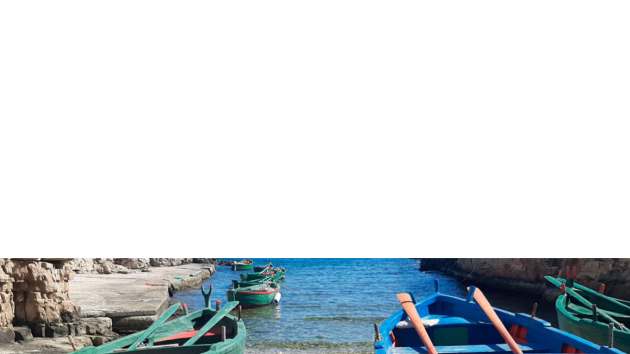
\includegraphics[width=\paperwidth]{background/template_169.pdf}}%
\begin{frame}[plain]
  \begin{center}
    \setlength{\parskip}{0pt}
    \vspace{10pt}
    {\Huge\bf Extra}
  \end{center}
\end{frame}
}

\begin{frame}
  \frametitle{\bf Correlation}
   \myy{} is not used as input feature to fully connected network (NN)
   classifier.\\ 
   Q: Why does the background get sculpted?\\
   A: Some of the input features are correlated to \myy{}.
  \begin{figure}
    \centering
    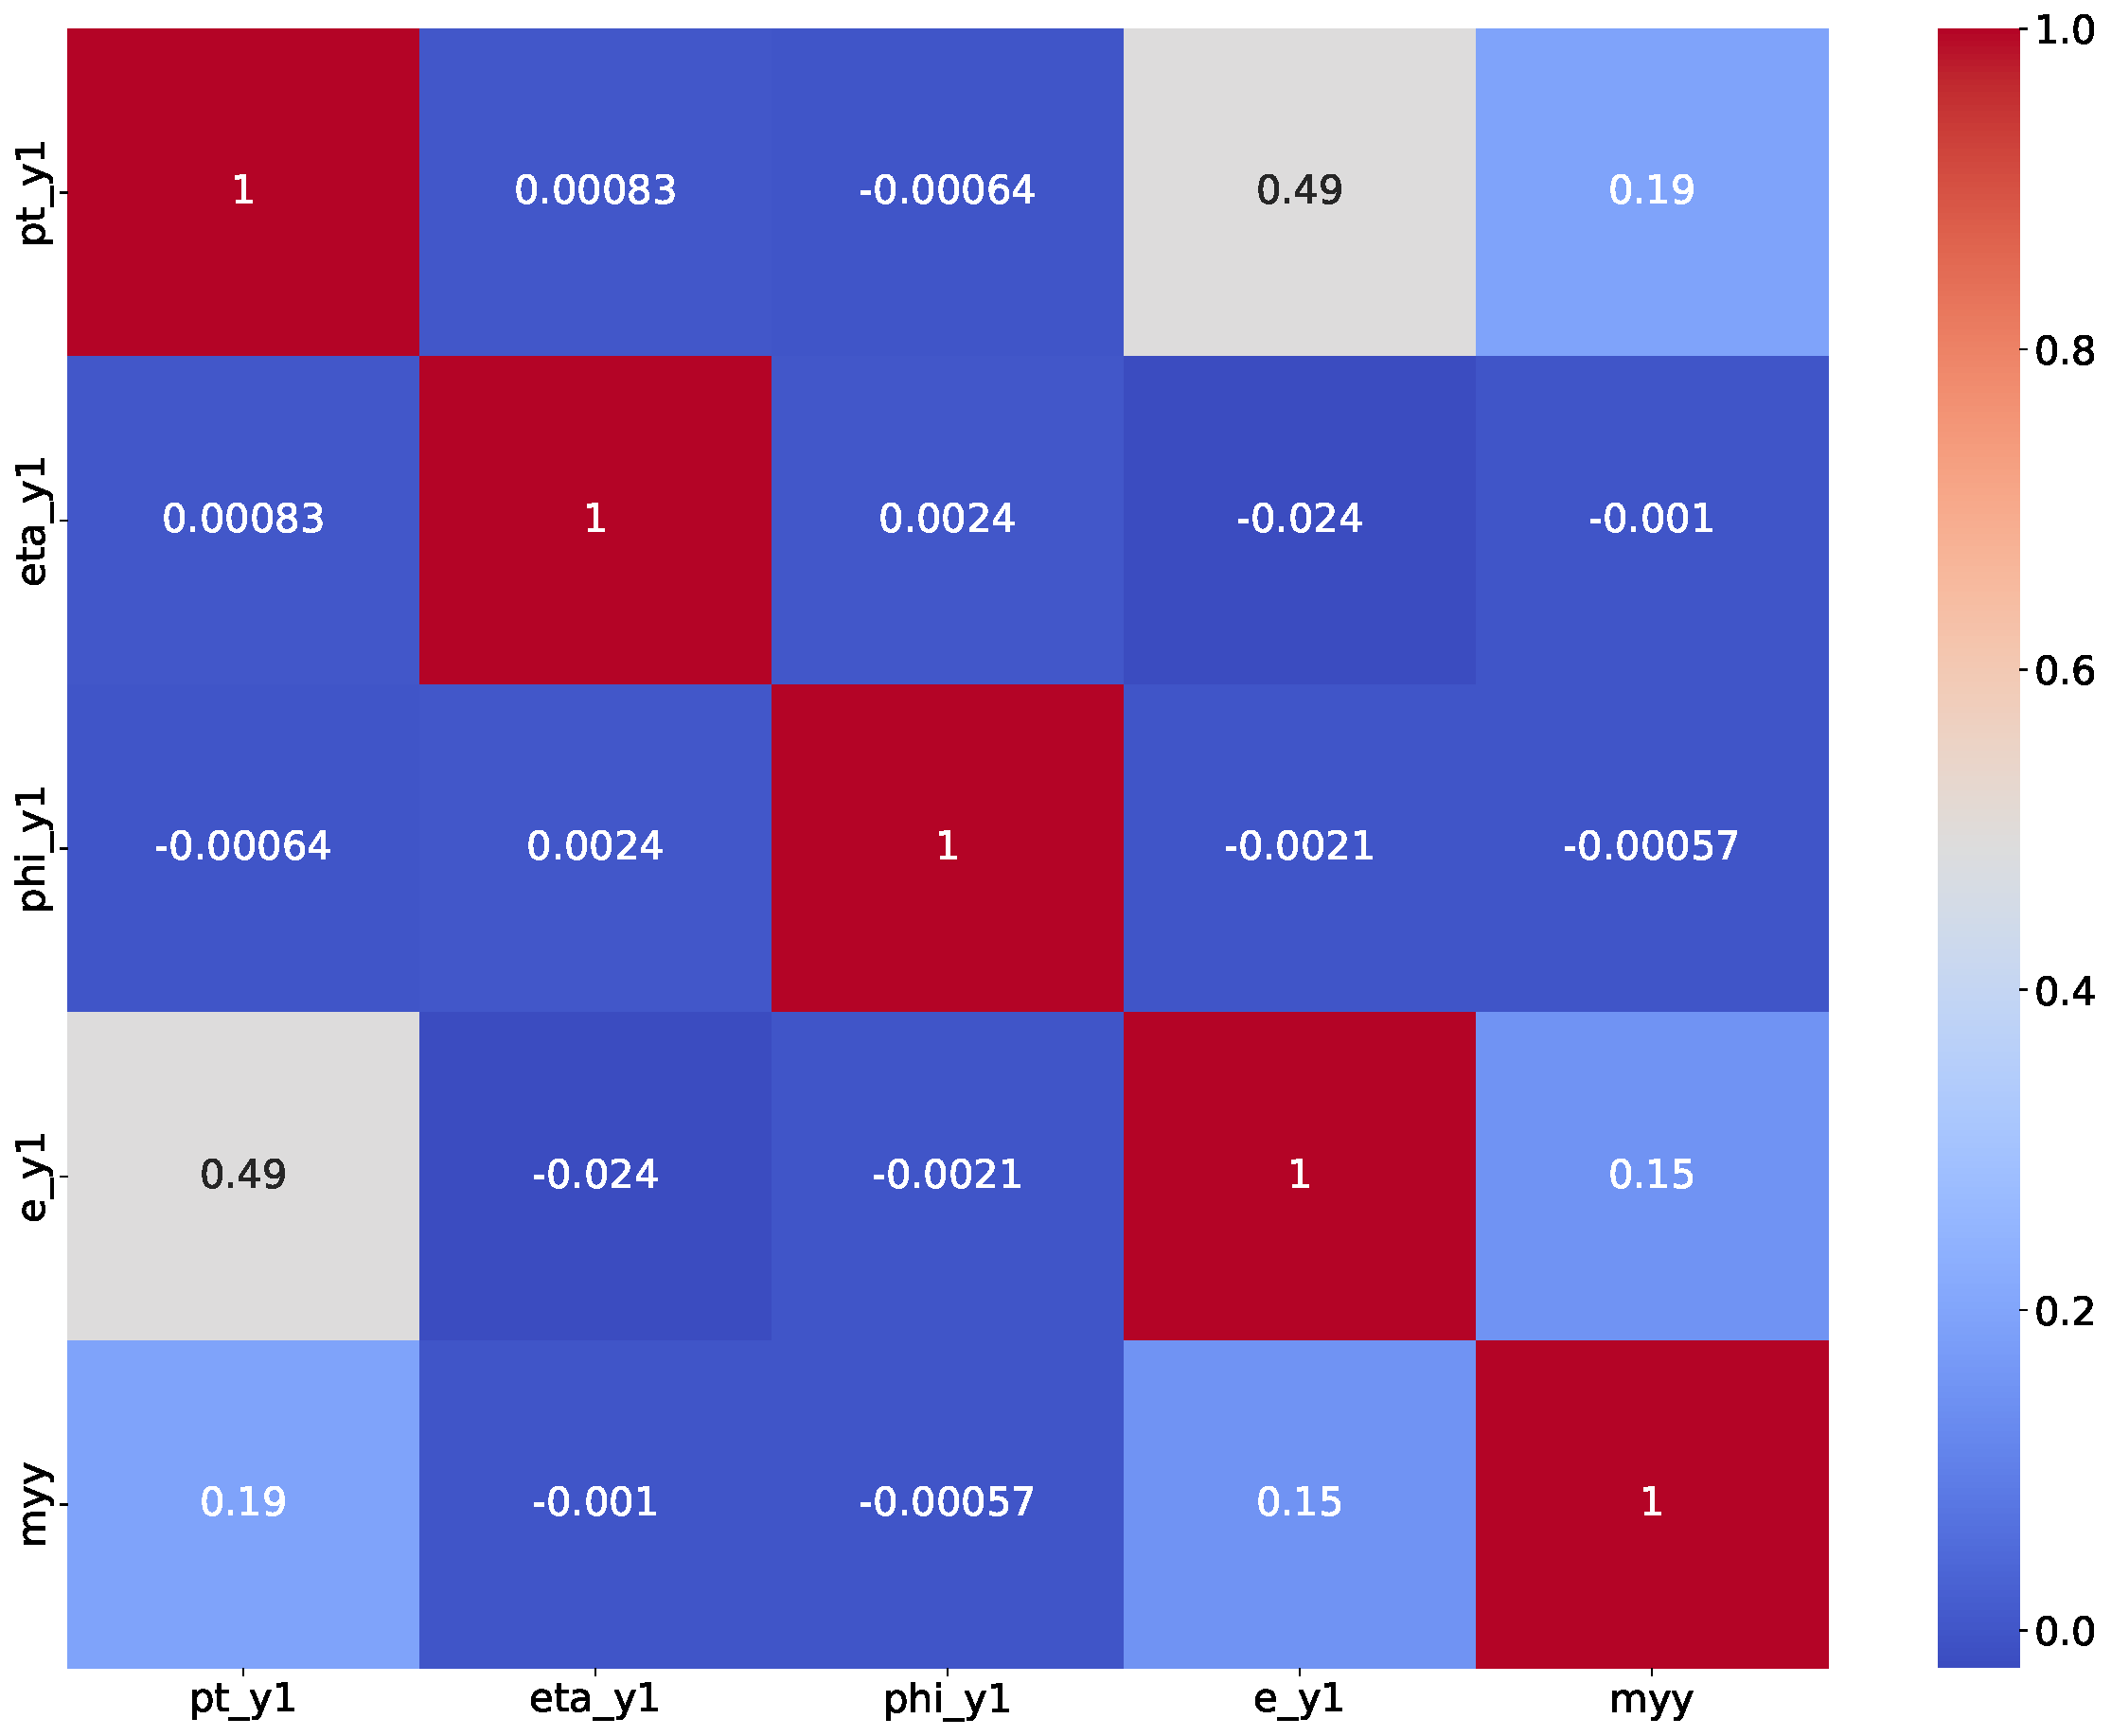
\includegraphics[width=0.5\textwidth]{figures/l2/lect_plots/corr_noscale.pdf}
  \end{figure}

\end{frame}

\backupend

\end{document}
